% ============================================================
%  WEATHER-FISH — Individual Contribution Report
%  OTH Amberg-Weiden  ·  Faculty of Electrical Engineering,
%  Media and Computer Science
%  Author: Fenil Ramani
%  Template follows: Technical_Report_Template_V5_0
%  Grounded in the original project definition: WEATHER-FISH
%  (Ramani, April 2026) — see content/WEATHER.pdf
% ============================================================

\documentclass[11pt, a4paper]{article}

% ── Packages ────────────────────────────────────────────────
\usepackage[T1]{fontenc}
\usepackage[utf8]{inputenc}
\usepackage[english]{babel}
\usepackage{lmodern}
\usepackage{microtype}
\usepackage{geometry}
\usepackage{fancyhdr}
\usepackage{titlesec}
\usepackage{abstract}
\usepackage{parskip}
\usepackage{booktabs}
\usepackage{tabularx}
\usepackage{array}
\usepackage{graphicx}
\usepackage{caption}
\usepackage{listings}
\usepackage{xcolor}
\usepackage{amsmath}
\usepackage{amssymb}
\usepackage{hyperref}
\usepackage{natbib}
\usepackage{enumitem}
\usepackage{float}
\usepackage{tikz}
\usetikzlibrary{arrows.meta, positioning, fit, backgrounds, calc}
\usepackage{ragged2e}

% ── Page geometry ───────────────────────────────────────────
\geometry{
  a4paper,
  left   = 2.5cm,
  right  = 2.5cm,
  top    = 2.4cm,
  bottom = 2.4cm,
  headheight = 14pt,
}

% ── Colours ─────────────────────────────────────────────────
\definecolor{gold}{RGB}{180,150,60}
\definecolor{myblue}{RGB}{70,110,170}
\definecolor{mygray}{RGB}{225,225,225}
\definecolor{codebg}{RGB}{245,245,245}
\definecolor{codegreen}{rgb}{0.0,0.5,0.0}
\definecolor{codegray}{rgb}{0.4,0.4,0.4}
\definecolor{codeblue}{rgb}{0.0,0.0,0.8}

% ── Running headers ─────────────────────────────────────────
\pagestyle{fancy}
\fancyhf{}
\renewcommand{\headrulewidth}{0.4pt}
\fancyhead[L]{\small Individual Report — Fenil Ramani}
\fancyhead[R]{\small WEATHER-FISH}
\fancyfoot[C]{\thepage}

% ── Section formatting ──────────────────────────────────────
\titleformat{\section}{\normalfont\large\bfseries}{\thesection}{1em}{}
\titleformat{\subsection}{\normalfont\normalsize\bfseries}{\thesubsection}{1em}{}
\titleformat{\subsubsection}{\normalfont\normalsize\itshape}{\thesubsubsection}{1em}{}
\titlespacing*{\section}{0pt}{8pt}{4pt}
\titlespacing*{\subsection}{0pt}{6pt}{2pt}

% ── Abstract formatting ─────────────────────────────────────
\renewenvironment{abstract}{%
  \small\begin{center}\textbf{A\footnotesize BSTRACT}\end{center}%
  \begin{quotation}
}{%
  \end{quotation}
}

% ── Code listing style ──────────────────────────────────────
\lstdefinestyle{pythonstyle}{
  backgroundcolor = \color{codebg},
  commentstyle    = \color{codegreen},
  keywordstyle    = \color{codeblue}\bfseries,
  stringstyle     = \color{red!60!black},
  basicstyle      = \ttfamily\footnotesize,
  breakatwhitespace = false,
  breaklines      = true,
  captionpos      = b,
  keepspaces      = true,
  numbers         = left,
  numbersep       = 5pt,
  numberstyle     = \tiny\color{codegray},
  showspaces      = false,
  showstringspaces= false,
  showtabs        = false,
  tabsize         = 2,
  frame           = single,
  rulecolor       = \color{black!20},
  language        = Python,
}

\hypersetup{
  colorlinks = true,
  linkcolor  = black,
  citecolor  = black,
  urlcolor   = black,
}

% ── TikZ node styles used by both diagrams ──────────────────
\tikzstyle{mine}   = [rectangle, rounded corners, draw=gold, very thick, fill=gold!15,
                       minimum height=0.9cm, text width=2.1cm, align=center, font=\small]
\tikzstyle{theirs} = [rectangle, rounded corners, draw=black!50, thick, fill=mygray,
                       minimum height=0.9cm, text width=2.1cm, align=center, font=\small]
\tikzstyle{flow}   = [rectangle, rounded corners, draw=myblue, thick, fill=myblue!10,
                       minimum height=0.8cm, text width=3.6cm, align=center, font=\small]
\tikzstyle{safety} = [rectangle, rounded corners, draw=gold, very thick, fill=gold!20,
                       minimum height=0.8cm, text width=3.6cm, align=center, font=\small]
\tikzstyle{ext}    = [rectangle, rounded corners, draw=myblue, thick, fill=myblue!8,
                       minimum height=0.9cm, text width=2.5cm, align=center, font=\small]
\tikzstyle{arr}    = [-{Stealth[length=2.2mm]}, thick]

% ── Layered-architecture styles (mine / teammates' / external) ──
\tikzstyle{layerMine}   = [rectangle, rounded corners, draw=gold, very thick, fill=gold!12,
                            minimum height=1.0cm, text width=7.2cm, align=center, font=\small,
                            inner sep=6pt]
\tikzstyle{layerTheirs} = [rectangle, rounded corners, draw=black!55, thick, fill=mygray,
                            minimum height=1.0cm, text width=7.2cm, align=center, font=\small,
                            inner sep=6pt]
\tikzstyle{layerExt}    = [rectangle, rounded corners, draw=myblue, thick, fill=myblue!8,
                            minimum height=1.0cm, text width=7.2cm, align=center, font=\small,
                            inner sep=6pt]
\tikzstyle{decision}    = [rectangle, rounded corners, draw=gold!70!black, thick, dashed,
                            fill=gold!5, text width=3.9cm, align=left, font=\scriptsize,
                            inner sep=5pt]

% ============================================================
\begin{document}
\justifying

% ── Title block ─────────────────────────────────────────────
\begin{center}
  \rule{\linewidth}{1.5pt}\\[6pt]
  {\Large\sc Weather-Fish: System Architecture, AI Integration, and Deployment}\\[4pt]
  \rule{\linewidth}{0.6pt}\\[6pt]
  {\small\sc Individual Contribution Report}\\[12pt]

  \textbf{Fenil Ramani}\\[2pt]
  \textit{Project Lead}\\[4pt]
  Faculty of Electrical Engineering, Media and Computer Science\\
  OTH Amberg-Weiden\\
  \texttt{f.ramani@oth-aw.de}\\[10pt]
  July 11, 2026
\end{center}

\vspace{6pt}

% ── Abstract ────────────────────────────────────────────────
\begin{abstract}
This report explains, in plain terms, what I personally built for WEATHER-FISH --- an
AI-driven weather app developed by a three-person team at OTH Amberg-Weiden. The project
brief names me as Project Lead, responsible for \textit{``system architecture, AI
integration, prompt engineering, and deployment''}, while my teammates Prasad Rajyguru
and Shubham Kushwaha handled the frontend/audio and the backend routes/scheduler. This
report covers only my part: the Context Engine that decides the tone of a report, the AI
model that writes the text, the safety-net fallback that keeps the app working when the AI
provider runs out of quota, the chat assistant built on top of it, the worldwide city
search, and the deployment to Hugging Face. Diagrams are included to make the design easy
to follow. The report also explains how my work connected to my teammates' work, and one
real integration mistake that came up and how I fixed it.
\end{abstract}

\vspace{2pt}
\noindent\textit{Keywords}\quad
Individual contribution $\cdot$ System architecture $\cdot$ AI integration $\cdot$
Prompt engineering $\cdot$ Fallback design $\cdot$ Deployment

\bigskip

% ============================================================
\section{Introduction}

WEATHER-FISH turns a plain weather app into one that writes and speaks a personalised
weather report, instead of just showing numbers on a screen. Reports are generated ahead of
time, so they play back instantly, and their wording changes automatically depending on
whether the weather is calm, dangerous, or great for outdoor plans \citep{weatherfish2026}.

The project brief splits this into three jobs (Table~\ref{tab:boundary}). My job, as
Project Lead, is \textit{``system architecture, AI integration, prompt engineering,
deployment''} \citep{weatherfish2026}. In the system flow diagram from the brief ---
\textit{Weather API~$\rightarrow$~Context Engine~$\rightarrow$~Prompt
Engineering~$\rightarrow$~AI Model~$\rightarrow$~TTS~$\rightarrow$~Storage~$\rightarrow$~
Playback} --- that means I built the three middle stages, plus the overall design that
connects every stage, plus getting the finished app online.

This report only covers my own work and how it connects to the rest of the team. It does
not describe my teammates' code in detail.

% ============================================================
\section{Who Did What}

\begin{table}[H]
  \centering
  \caption{Team responsibilities, exactly as written in the project brief
           \citep{weatherfish2026}. Only my row is explained further in this report.}
  \label{tab:boundary}
  \begin{tabularx}{\linewidth}{@{}lX@{}}
    \toprule
    \textbf{Team member} & \textbf{Job} \\
    \midrule
    \textbf{Fenil Ramani (me), Project Lead} & System architecture, AI integration,
      prompt engineering, deployment. \\[3pt]
    Prasad Rajyguru & Frontend, UI/UX, audio playback, user interaction. \\[3pt]
    Shubham Kushwaha & Backend, API integration, scheduler, storage. \\
    \bottomrule
  \end{tabularx}
\end{table}

Figure~\ref{fig:pipeline} shows the architecture as a cycle rather than a stack, because
that is what it actually is: the same six steps repeat automatically, once an hour, without
anyone touching the app. Gold steps are mine; grey steps were built by the rest of the team
(Table~\ref{tab:boundary}); the whole cycle runs inside the single container I deployed.

\begin{figure}[H]
  \centering
  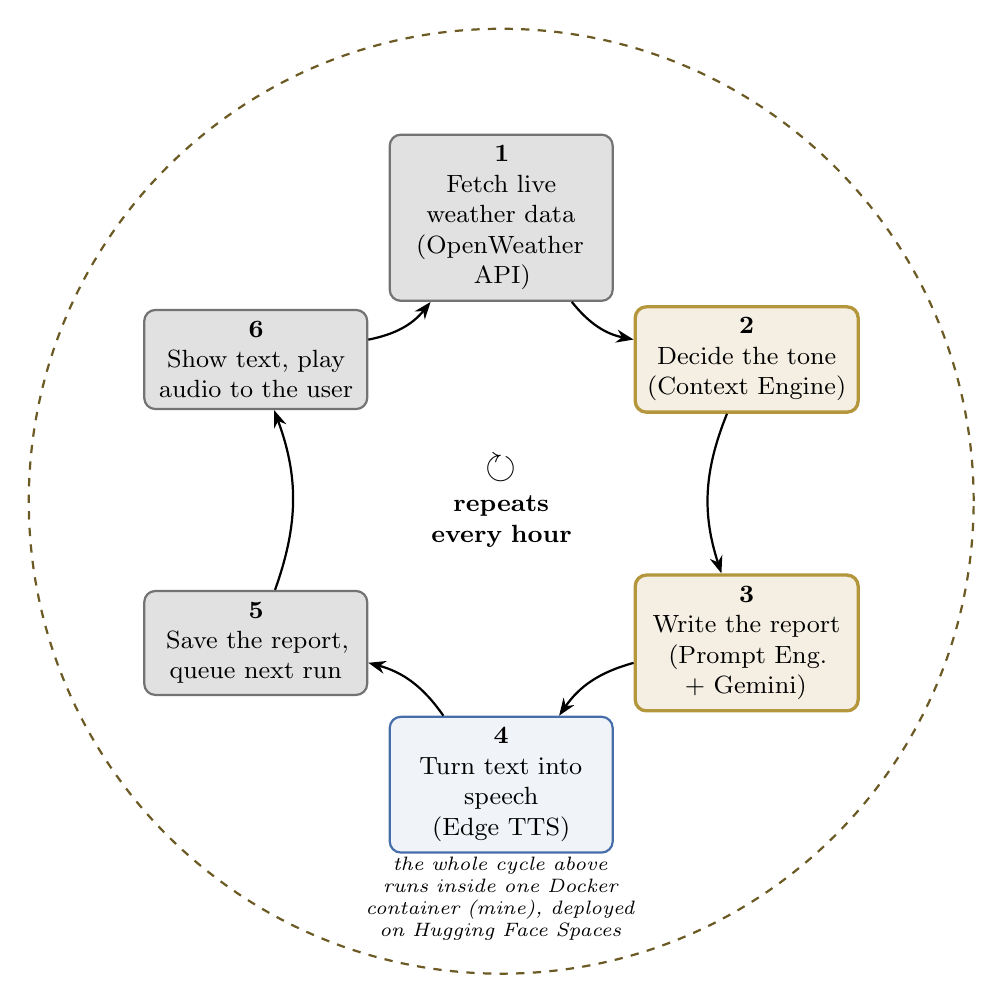
\begin{tikzpicture}[
      stage/.style={rectangle, rounded corners, thick, minimum height=1.15cm,
                     text width=2.55cm, align=center, font=\small, inner sep=4pt},
    ]
    \draw[gold!60!black, thick, dashed] (0,0) circle (6.0cm);
    \node[font=\scriptsize\itshape, align=center, text width=3.4cm]
         at (270:5.05) {the whole cycle above runs inside one Docker\\
                         container (mine), deployed on Hugging Face Spaces};

    \node[stage, draw=black!55, fill=mygray]          (n1) at (90:3.6)
      {\textbf{1}\\Fetch live weather data\\(OpenWeather API)};
    \node[stage, draw=gold, very thick, fill=gold!15] (n2) at (30:3.6)
      {\textbf{2}\\Decide the tone\\(Context Engine)};
    \node[stage, draw=gold, very thick, fill=gold!15] (n3) at (-30:3.6)
      {\textbf{3}\\Write the report\\(Prompt Eng.\ + Gemini)};
    \node[stage, draw=myblue, fill=myblue!8]          (n4) at (-90:3.6)
      {\textbf{4}\\Turn text into\\speech (Edge TTS)};
    \node[stage, draw=black!55, fill=mygray]          (n5) at (-150:3.6)
      {\textbf{5}\\Save the report,\\queue next run};
    \node[stage, draw=black!55, fill=mygray]          (n6) at (150:3.6)
      {\textbf{6}\\Show text, play\\audio to the user};

    \node[font=\small, align=center, text width=2.5cm] at (0,0)
      {{\Large$\circlearrowright$}\\[1pt]\textbf{repeats}\\\textbf{every hour}};

    \draw[arr] (n1) to[bend right=20] (n2);
    \draw[arr] (n2) to[bend right=20] (n3);
    \draw[arr] (n3) to[bend right=20] (n4);
    \draw[arr] (n4) to[bend right=20] (n5);
    \draw[arr] (n5) to[bend right=20] (n6);
    \draw[arr] (n6) to[bend right=20] (n1);
  \end{tikzpicture}
  \caption{The WEATHER-FISH cycle: one automated loop, triggered every hour by the
           scheduler. Gold = my steps; grey = built by the rest of the team; the dashed
           ring is the single Docker container the whole loop runs inside.}
  \label{fig:pipeline}
\end{figure}

% ============================================================
\section{What I Built}

\subsection{Context Engine: deciding the tone}

The brief says the Context Engine must look at weather severity, time of day, and user
preferences, and turn that into simple labels such as \textit{warning}, \textit{advisory},
or \textit{cheerful} \citep{weatherfish2026}. I built this as a small, rule-based Python
function. It does not use AI --- it uses plain if/else logic on temperature and rain data.
I made this choice on purpose: a storm warning should always be described as urgent, and a
rule always does that the same way, whereas an AI model might phrase it differently each
time.

\begin{lstlisting}[style=pythonstyle, caption={What the Context Engine outputs. This
  small object is then handed to the AI model as instructions.}]
{
  "severity": "warning", "time_of_day": "morning",
  "tone": "cautionary and urgent -- warn the user clearly",
  "highlights": ["current rainfall -- recommend an umbrella"],
}
\end{lstlisting}

\subsection{AI Model and Fallback: writing the report}

This is the core AI-integration task from the brief. I connect to Google Gemini and ask it
to write the report text, using the Context Engine's labels to set the tone (this is the
``prompt engineering'' part). The one thing I had to design around is quota: a free Gemini
account can only be used a limited number of times per day. If I only used one model, the
whole app would stop writing new reports once that daily limit was hit.

My fix was to try several models, one after another, and only fall back to a fixed,
no-AI template if every single one is out of quota. Figure~\ref{fig:fallback} shows this
as a simple flowchart.

\begin{figure}[H]
  \centering
  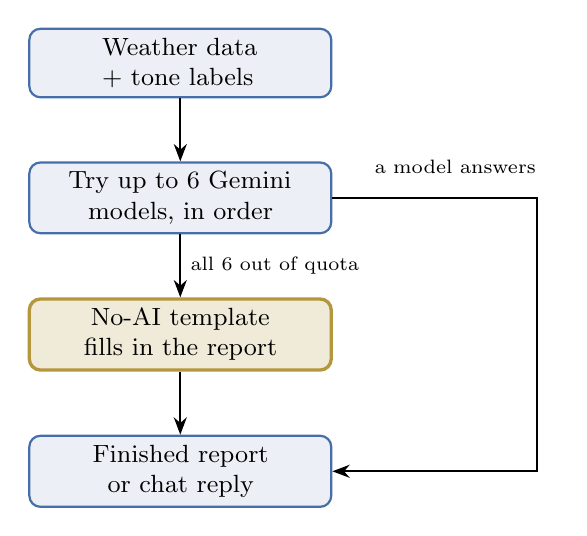
\begin{tikzpicture}[node distance=0.8cm]
    \node[flow] (input) {Weather data + tone labels};
    \node[flow, below=of input] (try) {Try up to 6 Gemini models, in order};
    \node[safety, below=of try] (fallback) {No-AI template fills in the report};
    \node[flow, below=of fallback] (out) {Finished report or chat reply};

    \draw[arr] (input) -- (try);
    \draw[arr] (try) -- node[right, font=\scriptsize, text width=2.5cm, align=left]
                          {all 6 out of quota} (fallback);
    \draw[arr] (fallback) -- (out);
    \draw[arr] (try.east) -- ++(2.6,0) coordinate (byp) |- (out.east);
    \node[font=\scriptsize, align=center, text width=2.4cm]
         at ($(try.east)!0.6!(byp)+(0,0.4)$) {a model answers};
  \end{tikzpicture}
  \caption{My fallback design: the app always finishes with a report, even if the AI
           model is completely unavailable. Gold boxes are the safety-net path.}
  \label{fig:fallback}
\end{figure}

\begin{lstlisting}[style=pythonstyle, caption={The six models I use, in the order I try
  them. Each one has its own separate daily quota.}]
MODELS = ["gemini-2.5-flash-preview-05-20", "gemini-2.5-flash",
          "gemini-2.0-flash", "gemini-2.0-flash-lite",
          "gemini-1.5-flash-001", "gemini-1.5-flash-8b-001"]
\end{lstlisting}

On top of this, I wrote three presenter personalities (Fisch, Merkel, Haftbefehl) as
prompt instructions, so the same weather data can be narrated in three very different
voices, plus a small randomised instruction that stops the AI from writing the same
opening sentence every time.

\subsection{Chat Assistant}

I reused the same Context Engine and the same model list to build a chat assistant, so it
always agrees with the report the user is already looking at. Its most useful feature does
not need AI at all: if a user asks something like \textit{``good for cycling today?''}, the
assistant checks rain chance, temperature, and wind speed directly against simple
thresholds and gives a clear yes/no answer. This means activity questions still work even
on a day when the AI quota is completely used up, in both German and English.

\subsection{Worldwide City Search}

The app originally only understood German postal codes. I changed this so any city in the
world can be searched: the frontend sends a search text to my backend, my backend asks a
geocoding service for matching cities, and returns them as a simple list. I picked an
identifier format (latitude\_longitude, e.g.\ \texttt{"22.3000\_70.8000"}) that did not
require changing how reports are already stored, so this upgrade did not break anything my
teammates had already built on the old German-only format.

\subsection{Deployment}

The last part of my job is deployment. I packaged the whole app --- backend, AI layer, and
the built frontend --- into one Docker container and put it on Hugging Face Spaces, so
anyone can open it in a browser without installing anything, matching the brief's goal.

% ============================================================
\section{Working with My Teammates}
\label{sec:collab}

Because my three AI stages sit between the other two teammates' stages, I made sure every
one of my endpoints returned a fixed, predictable shape of data, and treated that shape as
a promise to the rest of the team. For example, my city-search endpoint always returns a
list of \texttt{\{name, country, lat, lon, id\}} objects, and my report endpoint always
accepts \texttt{\{cities, zipcodes, language, hobbies\}}. This let my teammates build their
side without waiting for me to finish, or knowing how my AI code works internally.
Figure~\ref{fig:collab} shows the two places this handoff happens in practice.

\begin{figure}[H]
  \centering
  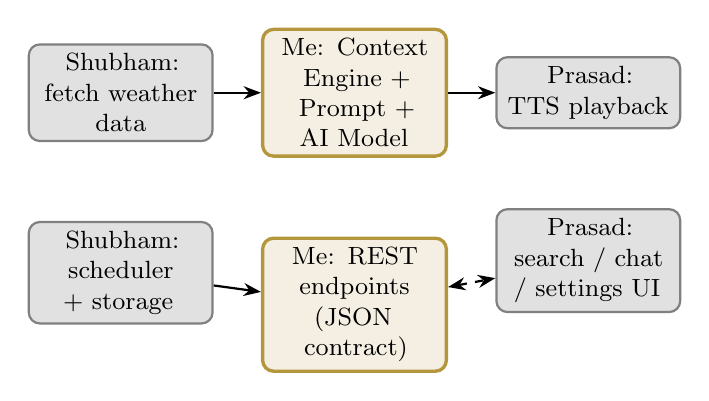
\begin{tikzpicture}[node distance=0.6cm and 0.6cm]
    \node[theirs] (s1) {Shubham:\\fetch weather data};
    \node[mine, right=of s1]   (f1) {Me: Context Engine +\\Prompt + AI Model};
    \node[theirs, right=of f1] (p1) {Prasad:\\TTS playback};

    \node[theirs, below=1.0cm of s1] (s2) {Shubham:\\scheduler + storage};
    \node[mine,   below=1.0cm of f1] (f2) {Me: REST endpoints\\(JSON contract)};
    \node[theirs, below=1.0cm of p1] (p2) {Prasad:\\search / chat / settings UI};

    \draw[arr] (s1) -- (f1);
    \draw[arr] (f1) -- (p1);
    \draw[arr] (s2) -- (f2);
    \draw[{Stealth[length=2.2mm]}-{Stealth[length=2.2mm]}, thick, dashed] (f2) -- (p2);
  \end{tikzpicture}
  \caption{How the three of us worked together. Top row: the data pipeline handoff
           (Shubham's weather data $\to$ my AI layer $\to$ Prasad's audio playback).
           Bottom row: the two-way interface contract between my REST endpoints and
           the scheduler/frontend code that calls them --- this is exactly where the
           Settings-page bug described below happened.}
  \label{fig:collab}
\end{figure}

That said, one mistake still slipped through. When I switched location IDs to the new
worldwide format, I updated the backend and one of the two search boxes in the frontend ---
but a second, older search box (on the Settings page) still only searched the old
German-only list, and nobody had noticed. Users typing a non-German city there simply saw
no results, even though the backend fully supported it. I only found this by testing the
live page myself, not by reviewing the backend code alone, because more than one search box
existed after several rounds of changes. Fixing it meant checking exactly which search box
the app actually used. Since then, I treat a change like this as ``done'' only after I have
checked every place that uses it --- not just the one I was thinking about when I made the
change.

We also deployed a new working version every couple of weeks instead of holding changes
until the end. This meant problems like the one above showed up quickly, instead of piling
up until a final integration week.

% ============================================================
\section{Results}

\begin{table}[H]
  \centering
  \caption{Outcomes from the work described in Section~3.}
  \label{tab:results}
  \begin{tabularx}{\linewidth}{@{}lX@{}}
    \toprule
    \textbf{What I built} & \textbf{Result} \\
    \midrule
    Six-model AI fallback & About $6\times$ more reports per day than using one AI model,
      for the same free quota. \\[3pt]
    No-AI template fallback & The app never shows an empty report, even when AI quota
      runs out completely. \\[3pt]
    Rule-based activity advice & Correct yes/no activity answers with zero AI calls, in
      German and English. \\[3pt]
    Worldwide city search & Any searchable city works now, not just German ZIP codes ---
      with no change needed to how reports are stored. \\[3pt]
    Deployment & The whole app runs from one container on Hugging Face Spaces. \\
    \bottomrule
  \end{tabularx}
\end{table}

% ============================================================
\section{What I Learned}

Building a safety net for the AI model mattered more than any single feature, because the
free daily quota ran out often during testing --- it was a normal, everyday problem, not a
rare edge case. I also learned that a design change is not really finished once my own code
works: the Settings-page mistake in Section~\ref{sec:collab} happened because I checked my
own change but not every place in the app that depended on it. I now double-check every
user of a changed interface, not just the one I had in mind.

% ============================================================
\section{Declaration of AI Tool Usage}

\noindent\textbf{Tools used:} Claude (Anthropic), used as a coding assistant inside my
editor.

\medskip
\noindent\textbf{Purpose:}
\begin{itemize}[noitemsep]
  \item Debugging help during backend development, e.g.\ tracing a type-checking error in
        the chat module, and diagnosing the Settings-page search bug described in
        Section~\ref{sec:collab}.
  \item Turning my own notes on what I built into clear, structured writing for this
        report, which I then reviewed and edited myself.
  \item \textit{Google Gemini} (part of the app I built, not a writing tool) is the AI
        model that writes the reports and chat replies described in Section~3.
\end{itemize}

\noindent I reviewed and tested every AI-assisted suggestion before using it. The ideas,
analysis, and conclusions in this report are my own.

% ============================================================
\bibliographystyle{plainnat}
\begin{thebibliography}{9}

\bibitem[Ramani(2026)]{weatherfish2026}
Ramani, F. (2026).
\newblock \textit{WEATHER-FISH — Project Definition}.
\newblock OTH Amberg-Weiden, internal project brief, April 2026.

\bibitem[Google(2024)]{google2024gemini}
Google~LLC (2024).
\newblock \textit{Gemini API Documentation}.
\newblock \url{https://ai.google.dev/gemini-api/docs}.

\bibitem[Tiangolo(2023)]{tiangolo2023fastapi}
Tiangolo, S. (2023).
\newblock \textit{FastAPI Documentation}.
\newblock \url{https://fastapi.tiangolo.com}.

\bibitem[OpenWeather(2024)]{openweather2024}
OpenWeather~Ltd (2024).
\newblock \textit{OpenWeather One Call API 3.0 and Geocoding API Documentation}.
\newblock \url{https://openweathermap.org/api/one-call-3}.

\end{thebibliography}

\end{document}
